\documentclass[11pt,a4paper]{article}

\usepackage{style2017}
\usepackage{hyperref}

\hypersetup{
    colorlinks =false,
    linkcolor=blue,
   linkbordercolor = 1 0 0
}
\newcounter{num}
\setcounter{num}{0}
\setcellgapes{1pt}

\newcommand{\nd}{n\oe{}ud~}
\newcommand{\nds}{n\oe{}uds~}
\begin{document}

\begin{NSI}
{Exercices}{Structure de données linéaires}
\end{NSI}


\stepcounter{num}
\section*{Exercice \thenum}

Écrire une fonction \textsf{recherche\_min} qui prend en paramètre un tableau de nombres non trié \textsf{t}, et qui renvoie l'indice de la première occurrence du minimum de ce tableau. Les tableaux seront représentés sous forme de liste Python.

\textbf{Quelques exemples}:

\textsf{recherche\_min([5])}

0

\textsf{recherche\_min([2,4,1])}

2

\textsf{recherche\_min([5,3,2,2,4])}

2


\stepcounter{num}
\section*{Exercice \thenum}

On considère la fonction \textsf{separe} ci-dessous qui prend en argument un tableau \textsf{tab} dont les éléments sont des 0 et des 1 et qui sépare les 0 des 1 en plaçant les 0 en début de tableau et les 1 à la suite.

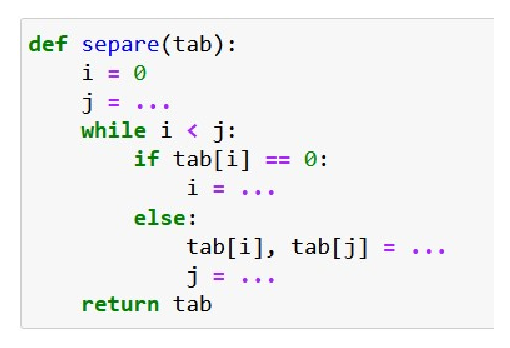
\includegraphics[scale=0.8]{../img/fct_separe.eps}

Compléter la fonction \textsf{separe} ci-dessus.

\textbf{Quelques exemples}:

\textsf{separe([1,0,1,0,1,0,1,0])}

\textsf{[0,0,0,0,1,1,1,1]}

\textsf{separe([1,0,0,0,1,1,0,1,1,0,1,0,1,1,1,0])}

\textsf{[0,0,0,0,0,0,0,1,1,1,1,1,1,1,1,1]}


\stepcounter{num}
\section*{Exercice \thenum}

Sur le réseau social \textbf{Tip Top}, on s'intéresse au nombre de "like" des abonnés. Les données sont stockées dans des dictionnaires où les clefs sont les pseudos et les valeurs correspondantes sont les nombres de "like" comme ci-dessous:

\begin{center}
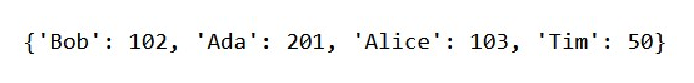
\includegraphics[scale=0.8]{../img/dico_like.eps}
\end{center}

Écrire une fonction \textsf{max\_dico} qui:
\begin{itemize}
\item Prend en paramètre un dictionnaire \textsf{dico} non vide dont les clés sont des chaines de caractères et les valeurs associées sont des entiers;
\item Renvoie un tuple dont:
\begin{itemize}
\item La première valeur est la clé du dictionnaire associée à la valeur maximale;
\item La seconde valeur est la première valeur maximale présente dans le dictionnaire.
\end{itemize}
\end{itemize}

\textbf{Quelques exemples}:

\textsf{max\_dico(\{'Bob':102,'Ada':201,'Alice':103,'Tim':50\})}

\textsf{('Ada',201)}

\textsf{max\_dico(\{'Alan':222,'Ada':201,'Eve':220,'Tim':50\})}

\textsf{('Alan',222)}


\stepcounter{num}
\section*{Exercice \thenum}

On souhaite manipuler des dates en Python. Il existe un module Date mais on ne va l'utiliser.

On considère qu'une date contient le jour, le mois et l'année. Par exemple, aujourd'hui nous sommes le 6 septembre 2022. On s'intéressera aux dates comprises entre les années 2000 et 2100.

L'objectif est de :
\begin{itemize}
\item créer des variables qui ont pour valeur une date.
\item créer des opérations sur les dates comme l'égalité ou la comparaison;
\item déterminer si une date est vide ou non;
\item déterminer si une date est valide;
\item afficher une date en utilisant une chaine de caractères
\end{itemize}


\begin{enumerate}
\item Donner différents types permettant de créer une date. On fera plusieurs propositions en précisant le type utilisé.

\item La fonction \textsf{est\_vide(d)} prend en paramètre une date \textsf{d} et renvoie un booléen affirmant si la d est vide ou non.
Écrire le code de cette fonction.

\item La fonction \textsf{est\_valide(d)} prend une date \textsf{d} en paramètre et renvoie un booléen qui affirme si la date \textsf{d} est correctement écrite, dans le bon type et le bon format et avec des valeurs cohérentes.
Écrire le code de cette fonction.

\item La fonction \textsf{egales} prend en paramètres deux dates et renvoie un booléen affirmant que les dates saisies sont les mêmes.
Écrire le code de cette fonction.

\item La fonction \textsf{est\_avant(d1,d2)} prend en paramètres deux dates \textsf{d1} et \textsf{d2} et renvoie un booléen affirmant que la date \textsf{d1} est plus ancienne que la date \textsf{d2}.
Écrire le code de cette fonction.

\item Créer une fonction d'affichage de date.
\end{enumerate}


\end{document}

